\section{Discussão Final}

\subsection{Comparativo Geral das Abordagens}

O trabalho evoluiu em seis estágios principais do lado Java (serial, v2, v3, v4,
v5, v6), cada um respondendo a uma limitação do estágio anterior, além de uma
implementação paralela em Erlang usada como ponto de comparação de modelo de
concorrência.

\textbf{Serial.}
A implementação sequencial estabeleceu a baseline: uma thread lê o CSV, calcula a
distância de cada ponto aos centróides e acumula os resultados. O perfil de execução
revelou que $\approx$82\% do tempo era gasto em parsing CSV
(\texttt{FloatingDecimal.parseDouble}, \texttt{String.split}), e apenas $\approx$8\%
em computação aritmética. Isso significa que o algoritmo em si é rápido; o gargalo
é a entrada de dados.

\textbf{Concorrente v2 (platform, virtual, hybrid).}
A paralelização da fase de atribuição (lotes de 5.000 pontos, pool de $N$ workers)
não trouxe ganho de tempo por iteração: o parsing CSV seguia sequencial na thread
principal, dominando o tempo total. Os microbenchmarks mostraram B2
$\approx$60 s/op para todas as variantes, idêntico ao serial. O macrobenchmark
revelou throughput de 1,6--4,6 exec/min dependendo do número de threads JMeter
e da variante de GC.

A exploração das três variantes foi útil para entender o comportamento de cada
modelo de thread. A variante hybrid foi a mais reveladora: ao usar uma virtual thread
como coordenadora, o parsing CSV ficou invisível ao profiler --- porque a thread
suspende durante I/O em vez de consumir CPU. Isso confirmou que o gargalo não estava
na coordenação dos workers, mas na leitura do arquivo em si.

\textbf{Concorrente v3 (dados em memória).}
Carregar o dataset inteiro em \texttt{double[][]} antes do loop de iterações
eliminou o parsing CSV das medições. B2 caiu de $\approx$60 s para $\approx$1{,}6 s
($\approx$37$\times$); o throughput saltou de $\approx$1,6 para $\approx$52
exec/min com 1 thread JMeter. O perfil não registrou nenhum evento de leitura de
arquivo durante o clustering. O custo foi o aumento do heap de $\approx$250 MB
para $\approx$2{,}7 GB.

\textbf{Concorrente v4 (concorrência estruturada).}
A v4 substitui o par \texttt{ExecutorService} + \texttt{CountDownLatch} da v3
por \texttt{StructuredTaskScope} e \texttt{ScopedValue} (JEP 480/446), corrigindo uma
lacuna estrutural real: exceções lançadas dentro de uma tarefa de worker, antes
sem canal de propagação de volta à coordenadora, passam a propagar corretamente
via \texttt{scope.join()}, que também cancela subtarefas irmãs automaticamente.
O preço é um aumento modesto no custo por iteração (B2: 1{,}60 s $\to$ 1{,}98 s,
$\approx$24\%) e no throughput (52,5--62,3 $\to$ 45,8--52,0 exec/min), atribuído
à imaturidade de compilação das APIs de \textit{preview}. O confinamento local
por tarefa permanece inalterado e validado por JCStress.

\textbf{Concorrente v5 (fork/join).}
A v5 troca o particionamento fixo em $N$ chunks por divisão-e-conquista
recursiva com \texttt{RecursiveTask} e \textit{work-stealing}. Os números ficam
muito próximos aos da v4 (B2 = 1{,}78 s; throughput 46,4--52,4 exec/min) --- o
dataset uniforme deste trabalho não oferece o desbalanceamento entre partições
que o \textit{work-stealing} precisaria para mostrar vantagem real. O achado
mais relevante é a variância elevada de B1 ($\pm$16{,}08 s), ecoando o mesmo
efeito já visto na v2-virtual: pools de tarefas pensados para trabalho que
cede o processador introduzem ruído de escalonamento em cargas puramente
aritméticas que nunca bloqueiam.

\textbf{Spark (v6, processamento distribuído).}
A v6 abandona o modelo de memória compartilhada em favor de um
\texttt{Dataset<Row>} particionado gerenciado pelo Spark, com
\texttt{mapToPair}+\texttt{reduceByKey} por iteração e broadcast do snapshot de
centróides. Nem JMH, nem JMeter, nem JCStress se aplicam a este modelo; a
métrica usada foi tempo de parede. O tempo por iteração aproximado
($\approx$3{,}46 s no CSV; $\approx$4{,}43 s no Parquet) fica acima do B2 de
v3--v5 --- o custo de coordenação distribuída supera o benefício em um dataset
que cabe confortavelmente em uma única máquina. O achado mais interessante foi
contraintuitivo: o Parquet, formato colunar e comprimido, foi
$\approx$28\% \textit{mais lento} que o CSV bruto nesta carga, pela sobrecarga
de decodificação de dicionário/delta por linha. O cache do Spark também expôs
um modo de falha ausente nas versões single-JVM: sob pressão de memória,
partições não cacheadas são silenciosamente relidas/reparseadas em vez de
causar um erro explícito.

\textbf{Erlang concorrente (modelo de atores, dados em memória).}
Esta implementação parte do mesmo ponto que a v3 (dados em memória) e não foi
estendida para acompanhar v4--v6, que são extensões específicas do lado Java;
a comparação a seguir é sempre contra a v3. Distribui chunks entre 16 workers
BEAM, sem memória compartilhada. O custo por
iteração ficou em $\approx$21{,}3 s ($\approx$66$\times$ acima do Java v3 --- ver Tabela~\ref{tab:bench-erlang-vs-v3}). O gargalo é
a aritmética por ponto: B3 e B4 são 113--165$\times$ mais lentos que em Java,
pois a BEAM desempacota floats de binários sem vetorização SIMD. Os schedulers
operaram a 45{,}7\% de utilização — a redução centralizada serializa parte de
cada iteração.

A Tabela~\ref{tab:comparativo-geral} resume os principais números de cada abordagem.

\begin{table}[H]
\centering
\small
\begin{tabular}{lrrrr}
\hline
\textbf{Abordagem} & \textbf{B2 (s/op)} & \textbf{Throughput 1t} & \textbf{Throughput 16t} & \textbf{Heap pico} \\
\hline
Serial             & 60{,}05 & 1{,}56/min\textsuperscript{*} & 4{,}66/min\textsuperscript{*} & $\approx$250 MB \\
v2-platform        & 60{,}69 & 1{,}65/min & 4{,}49/min & $\approx$250 MB \\
v2-virtual         & 71{,}61 & 1{,}62/min & 4{,}55/min & $\approx$250 MB \\
v2-hybrid          & 60{,}44 & 1{,}60/min & 4{,}53/min & $\approx$250 MB \\
v3                 &  1{,}60 & 52{,}5/min & 62{,}3/min & $\approx$2{,}7 GB \\
v4                 &  1{,}98 & 45{,}8/min & 52{,}0/min & $\approx$2{,}76 GB \\
v5                 &  1{,}78 & 46{,}4/min & 52{,}4/min & $\approx$2{,}56 GB \\
v6-csv             & 3{,}46\textsuperscript{\ddag} & N/A\textsuperscript{\ddag} & N/A\textsuperscript{\ddag} & $\approx$3{,}89 GB \\
v6-parquet         & 4{,}43\textsuperscript{\ddag} & N/A\textsuperscript{\ddag} & N/A\textsuperscript{\ddag} & $\approx$3{,}99 GB \\
Erlang (16 workers)& 21{,}27\textsuperscript{\dag} &     N/A    &     N/A    & $\approx$1{,}75 GB \\
\hline
\end{tabular}
\caption{Comparativo geral entre abordagens (B2 = custo por iteração; throughput = exec/min, JMeter G1GC exceto v3--v5 com ParallelGC; Erlang sem macrobenchmark HTTP; v6 sem JMH/JMeter, ver texto).
\textsuperscript{*}Serial: $N$ instâncias independentes executadas em paralelo pelo JMeter (sem concorrência interna); ver Tabela~\ref{tab:jmeter-serial-java}.
\textsuperscript{\dag}Erlang B2 estimado como B1\,/\,\texttt{maxIter} (106.344{,}7\,ms\,÷\,5\,÷\,1000); sem benchmark B2 dedicado.
\textsuperscript{\ddag}v6: sem JMH dedicado; B2 estimado como tempo de parede total $\div$ 10 iterações
(ver Tabela~\ref{tab:wallclock-v6} na Seção~\ref{sec:spark}); sem macrobenchmark JMeter --- Spark
não foi projetado para atender chamadas concorrentes de alta frequência.}
\label{tab:comparativo-geral}
\end{table}

\begin{figure}[H]
    \centering
    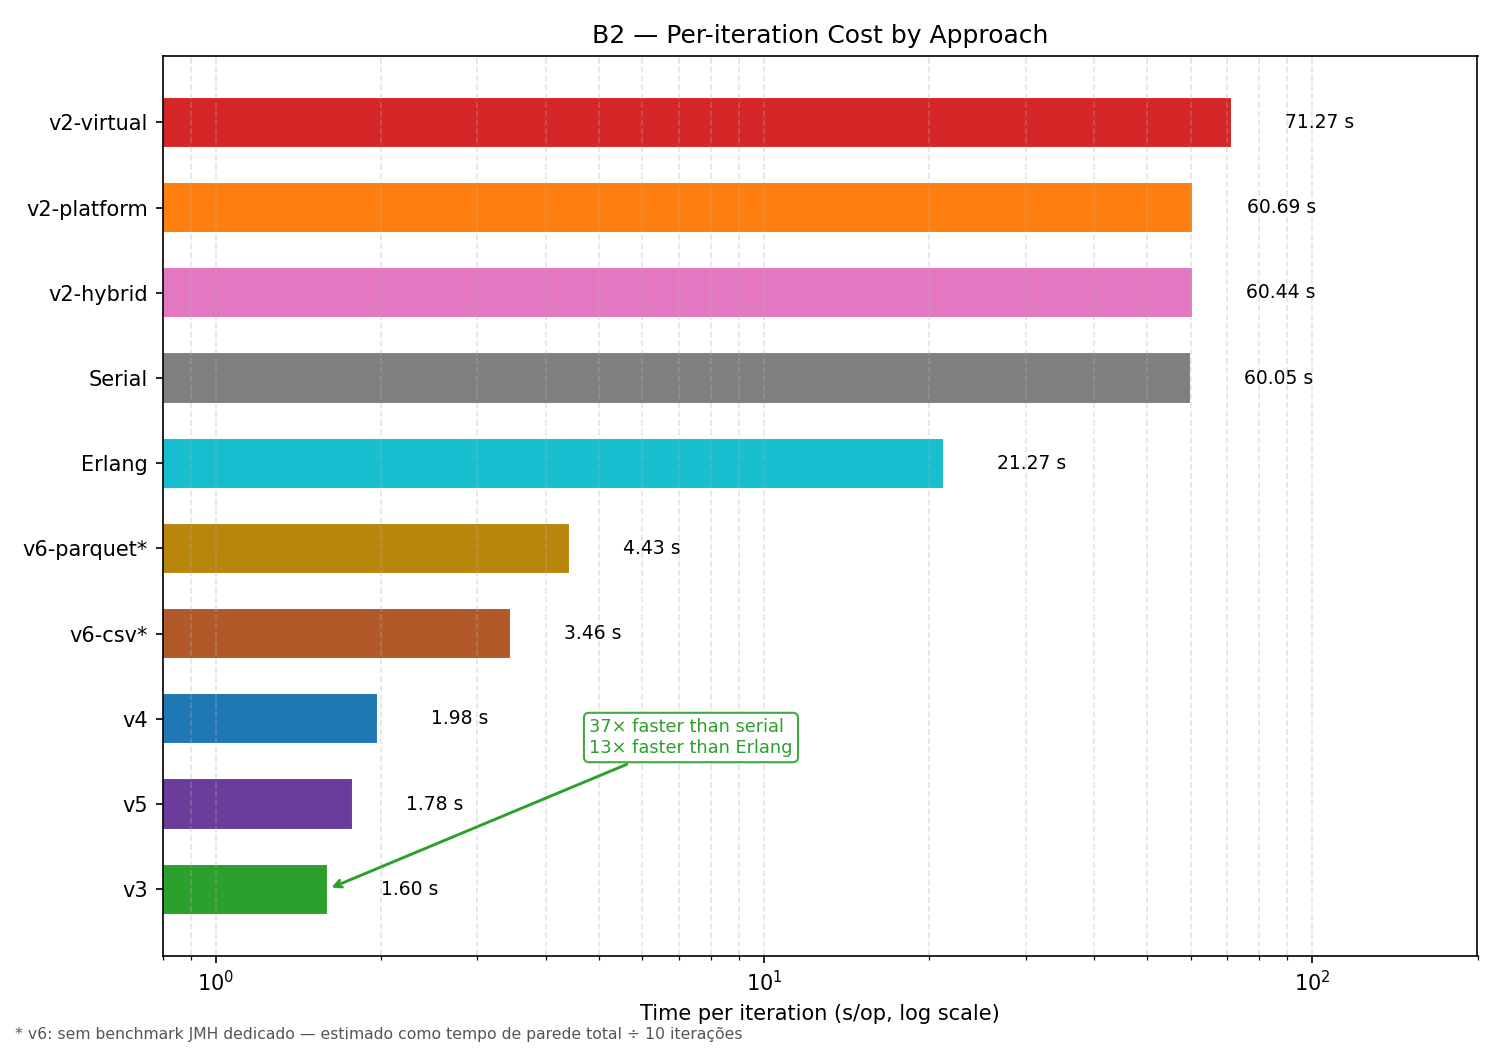
\includegraphics[width=0.85\textwidth]{img/charts/chart1_b2_cost}
    \caption{Custo por iteração (B2) em escala logarítmica, todas as abordagens.
             As variantes v2 e Serial ficam acima de 60 s/op, dominadas pelo
             parsing CSV. Erlang fica em 21{,}27 s/op ($\approx$13$\times$
             acima da v3) pelo custo aritmético da BEAM sem vetorização SIMD.
             v6-csv e v6-parquet (marcadas com {*}) não têm B2 dedicado ---
             o valor mostrado é o tempo de parede total dividido por 10
             iterações (ver Tabela~\ref{tab:wallclock-v6} na
             Seção~\ref{sec:spark}) --- e ainda assim ficam acima de v3, v4 e
             v5, que caem para a faixa de 1{,}6--2,0 s/op ao eliminar a
             coordenação distribuída. v3 segue sendo a mais rápida, $37\times$
             mais rápida que o Serial.}
    \label{fig:chart-b2-cost}
\end{figure}

O \texttt{chart2\_macro\_throughput.png} (Seção~\ref{sec:concurrent-x}) cobre
apenas Serial, v2 e v3 e foi mantido como está. A Figura~\ref{fig:chart-throughput-v3-v5}
é um gráfico novo e independente, comparando diretamente v3, v4 e v5 --- as
três únicas versões com macrobenchmark no mesmo coletor (ParallelGC), o que
torna a comparação direta sem ressalvas de GC.

\begin{figure}[H]
    \centering
    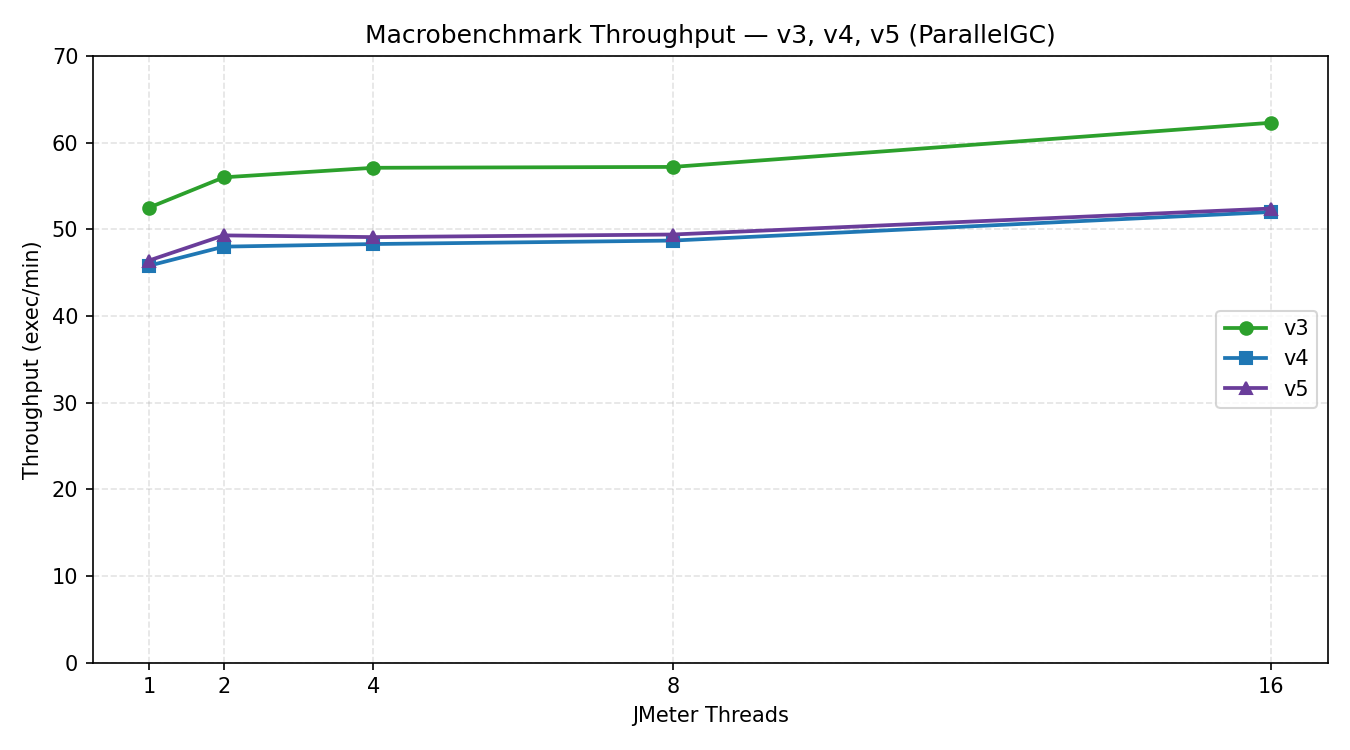
\includegraphics[width=0.85\textwidth]{img/charts/chart5_throughput_v3_v5}
    \caption{Throughput (execuções/min) por número de threads JMeter --- v3,
             v4 e v5, todas com ParallelGC. v4 e v5 ficam muito próximas entre
             si e abaixo da v3 em todos os níveis de carga, consistente com o
             aumento de custo por iteração (B2) discutido nas
             Seções~\ref{sec:structured} e~\ref{sec:forkjoin}. v6 não aparece
             neste gráfico --- não há macrobenchmark JMeter para o Spark (ver
             Seção~\ref{sec:spark}).}
    \label{fig:chart-throughput-v3-v5}
\end{figure}

\subsection{Pontos Positivos e Negativos de Cada Abordagem}

\subsubsection*{Serial}

\textbf{Positivos.}
Simples de implementar e depurar. Ausência de condições de corrida por definição.
Baixo consumo de memória. Serve como baseline clara para medir ganhos das versões
concorrentes.

\textbf{Negativos.}
Subutiliza processadores multi-core. A thread principal acumula os dois papéis
(I/O e computação) sem possibilidade de sobreposição.

\subsubsection*{v2 --- Concorrência com Lotes e Futures}

\textbf{Positivos.}
Paraleliza a fase computacionalmente intensiva (atribuição de pontos a centróides)
sem exigir sincronização explícita, graças à acumulação local por worker. A
estrutura de \texttt{Future.get()} fornece garantia de happens-before clara. A
variante hybrid demonstrou que virtual threads são adequadas para coordenadores
que alternam entre I/O e espera.

\textbf{Negativos.}
O parsing CSV sequencial na thread principal continua sendo o gargalo, tornando o
ganho da paralelização invisível no tempo de parede. A criação de objetos
\texttt{List.copyOf} e \texttt{PartialResult} por lote gera pressão de GC.
A virtual thread em tarefas CPU-bound de curta duração introduz variância elevada
no JMH (até $\pm$260 s), pois o \texttt{ForkJoinPool} não foi projetado para
tarefas que nunca bloqueiam.

\subsubsection*{Erlang --- Concorrência por Atores}

\textbf{Positivos.}
Race conditions são impossíveis por construção: processos não compartilham memória,
eliminando a necessidade de locks, atomics ou \texttt{volatile}. O GC é por
processo e sem pausas globais: nenhum stop-the-world afeta todos os workers
simultaneamente. Workers de longa duração mantêm os chunks em seus heaps locais
sem overhead de cópia, graças à semântica de referência dos binários grandes da
BEAM. O modelo de atores escala naturalmente para clusters distribuídos sem
mudança de paradigma.

\textbf{Negativos.}
A aritmética por ponto é 113--165$\times$ mais lenta que em Java: a BEAM
desempacota floats de binários elemento a elemento sem geração de código SIMD.
Os schedulers operaram a 45{,}7\% de utilização: a redução centralizada no processo
principal (\texttt{collect\_partial} + recompute) é um gargalo serial que mantém
os workers ociosos $\approx$54\% do tempo. A reconstrução de listas de somas via
\texttt{update\_nth} gerou 2{,}1 milhões de coletas GC por alocação excessiva de
células de lista --- custo inexistente em Java, que acumula em arrays mutáveis
locais. A ausência de servidor HTTP inviabilizou a comparação de throughput com
JMeter nas mesmas condições das versões Java.

\subsubsection*{v3 --- Dados em Memória com CountDownLatch}

\textbf{Positivos.}
Elimina o I/O das iterações, revelando o verdadeiro custo computacional do algoritmo.
A divisão em $N$ chunks fixos é mais simples que a criação dinâmica de lotes:
sem \texttt{List.copyOf}, sem \texttt{Future} por lote. \texttt{CountDownLatch}
é mais direto que coletar e iterar sobre uma lista de \texttt{Future}s. O
\texttt{KMeansSampler} com \texttt{sharedPoints} estático permite que múltiplos
threads JMeter compartilhem os dados sem alocar múltiplos GBs por thread.

\textbf{Negativos.}
O dataset inteiro precisa caber na heap ($\approx$1{,}75 GB para $\approx$5{,}75
milhões de pontos com 38 features). Isso inviabiliza a abordagem para datasets
maiores sem particionamento externo. O tempo de inicialização (leitura única do
CSV) não é contabilizado nas métricas, o que pode ser enganoso se o processo for
reiniciado frequentemente.

\subsubsection*{v4 --- Concorrência Estruturada}

\textbf{Positivos.}
Corrige uma lacuna estrutural real da v3: exceções de worker agora propagam
corretamente via \texttt{scope.join()}, com cancelamento automático de
subtarefas irmãs. \texttt{ScopedValue} substitui a passagem de centróides por
parâmetro com uma alternativa mais segura que \texttt{ThreadLocal} para virtual
threads filhas. O confinamento local por tarefa é preservado sem alterações e
segue validado por JCStress.

\textbf{Negativos.}
Custo mensurável em relação à v3: B2 sobe $\approx$24\% (1{,}60 s $\to$
1{,}98 s) e o throughput cai em todos os níveis de carga testados. As APIs de
\textit{preview} exigem \texttt{--enable-preview} em toda a cadeia de build e
execução (compilação, JMH, JCStress, JMeter).

\subsubsection*{v5 --- Fork/Join}

\textbf{Positivos.}
Introduz \textit{work-stealing} a nível de tarefa: divisão recursiva por
limiar permite que threads ociosas roubem subtarefas de outras, vantagem
estrutural em cargas desbalanceadas entre partições. B2 melhora levemente
frente à v4 (1{,}78 s).

\textbf{Negativos.}
Sem ganho aparente neste dataset uniforme --- números de throughput quase
idênticos aos da v4. A variância de B1 ($\pm$16{,}08 s) é a maior desde a
v2-virtual, mesmo efeito de ruído de agendamento em tarefas CPU-bound sobre
\texttt{ForkJoinPool}. Nenhum teste de sensibilidade ao limiar de divisão foi
realizado.

\subsubsection*{v6 --- Spark (Processamento Distribuído)}

\textbf{Positivos.}
Modelo de programação radicalmente diferente das versões anteriores
(transformações distribuídas sobre um \texttt{Dataset} particionado em vez de
threads coordenadas sobre memória compartilhada), relevante para cargas que
não cabem em uma única máquina. \texttt{mapToPair}+\texttt{reduceByKey}
expressa o mesmo padrão de acumulação local das versões anteriores em um
paradigma declarativo.

\textbf{Negativos.}
Mais lento que v3--v5 neste dataset, que cabe confortavelmente em memória numa
única máquina --- o overhead de coordenação distribuída não se paga nesta
escala. JMH, JMeter e JCStress não se aplicam, reduzindo a comparabilidade
direta com as versões anteriores. Sob pressão de memória, o cache degrada
silenciosamente para recomputação em vez de falhar de forma explícita (ao
contrário da v3, que ou cabe no heap ou lança \texttt{OutOfMemoryError}).
Contraintuitivamente, o formato Parquet foi $\approx$28\% mais lento que o CSV
nesta carga.

\subsection{Lições Aprendidas}

\textbf{Medir antes de paralelizar.}
O JFR mostrou que $\approx$82\% do tempo serial era parsing CSV. Paralelizar apenas o
loop aritmético ($\approx$8\% do total) dificilmente produziria ganho perceptível sem
antes eliminar o gargalo de I/O.

\textbf{Gargalos migram.}
Com o I/O eliminado na v3, o gargalo passou a ser \texttt{squaredDistance} e
\texttt{closestCentroid}. Em iterações futuras, esse é o ponto a otimizar
(SIMD, vetorização, redução de dimensionalidade).

\textbf{Virtual threads não são bala de prata para CPU-bound.}
Virtual threads brilham com bloqueio I/O, liberando o carrier para reuso.
Em tarefas puramente aritméticas, não oferecem vantagem sobre platform threads
e podem introduzir variância de escalonamento indesejada.

\textbf{Acumulação local elimina sincronização.}
O padrão map-reduce local — cada worker acumula em arrays próprios, a thread
coordenadora reduz no final — evitou locks, atomics e \texttt{volatile}.
O JCStress confirmou a ausência de race conditions nas operações reais e sua
presença ao remover a proteção (JCS3, JCS4).

\textbf{O modelo de atores não é universal.}
K-Means é CPU-bound com comunicação mínima entre iterações — perfil que favorece
memória compartilhada. O modelo de atores Erlang brilha em sistemas distribuídos,
I/O intensivo e alta disponibilidade, onde o isolamento de processos é vantagem
estrutural, não custo.

\textbf{Robustez estrutural tem custo mensurável.}
A v4 trocou uma lacuna real de tratamento de erro (exceção de worker
silenciosamente mascarada na v3) por um aumento de $\approx$24\% no custo por
iteração --- APIs mais seguras (\texttt{StructuredTaskScope},
\texttt{ScopedValue}) não são gratuitas enquanto ainda são \textit{preview}.

\textbf{\textit{Work-stealing} não ajuda cargas uniformes.}
A v5 não superou a v4 neste dataset sintético e bem distribuído entre
partições --- \textit{work-stealing} só compensa seu overhead de agendamento
quando há desbalanceamento real de carga, o que não é o caso aqui.

\textbf{Mudar o modelo de execução muda o cálculo de custo-benefício.}
O Spark (v6) foi mais lento que todas as versões Java de memória compartilhada
nesta escala --- o overhead de coordenação distribuída (serialização,
broadcast, gerenciamento de partições) só se paga quando o dataset não cabe
em uma única máquina.

\textbf{Formato de armazenamento também é uma variável de desempenho.}
Contra a intuição de que Parquet (colunar, comprimido) seria mais rápido que
CSV, ele foi $\approx$28\% mais lento nesta carga --- o custo de decodificação
de dicionário/delta por linha superou a economia de I/O bruto. Mais uma
confirmação da lição "medir antes de assumir".

\textbf{Sistemas distribuídos falham de formas que sistemas single-JVM não falham.}
Sob pressão de memória, o cache do Spark degrada silenciosamente para
recomputação em vez de lançar um erro explícito --- ao contrário da v3, onde o
dataset ou cabe no heap ou a JVM falha de forma visível.
